% Векторизация.
\newpage
\section*{Глава 5. Методы векторизации кода} % выключить номер главы
\addcontentsline{toc}{section}{Глава 5. Методы векторизации кода} % но добавить ее в оглавление
\addtocounter{section}{1}                                                    % а теперь и счетчик продвинуть
\setcounter{subsection}{0}
\setcounter{figure}{0}
\setcounter{equation}{0}
\setcounter{table}{0}
\setcounter{theorem}{0}
\setcounter{lemma}{0}
\setcounter{definition}{0}

%---------------------------------------------------------------------------------------------------
% 5.1 - AVX-512

%---------------------------------------------------------------------------------------------------
% 5.2 - композиция в виде плоских циклов

%---------------------------------------------------------------------------------------------------
% 5.3 - плоский цикл

%---------------------------------------------------------------------------------------------------
% 5.4 - вынос маловероятных регионов

%---------------------------------------------------------------------------------------------------
% 5.5 - слияние

%---------------------------------------------------------------------------------------------------
% 5.6 - объединение и комбинирование

%---------------------------------------------------------------------------------------------------
% 5.7 - гнезда циклов

%---------------------------------------------------------------------------------------------------
% Выводы. 

\begin{figure}[ht]
\centering
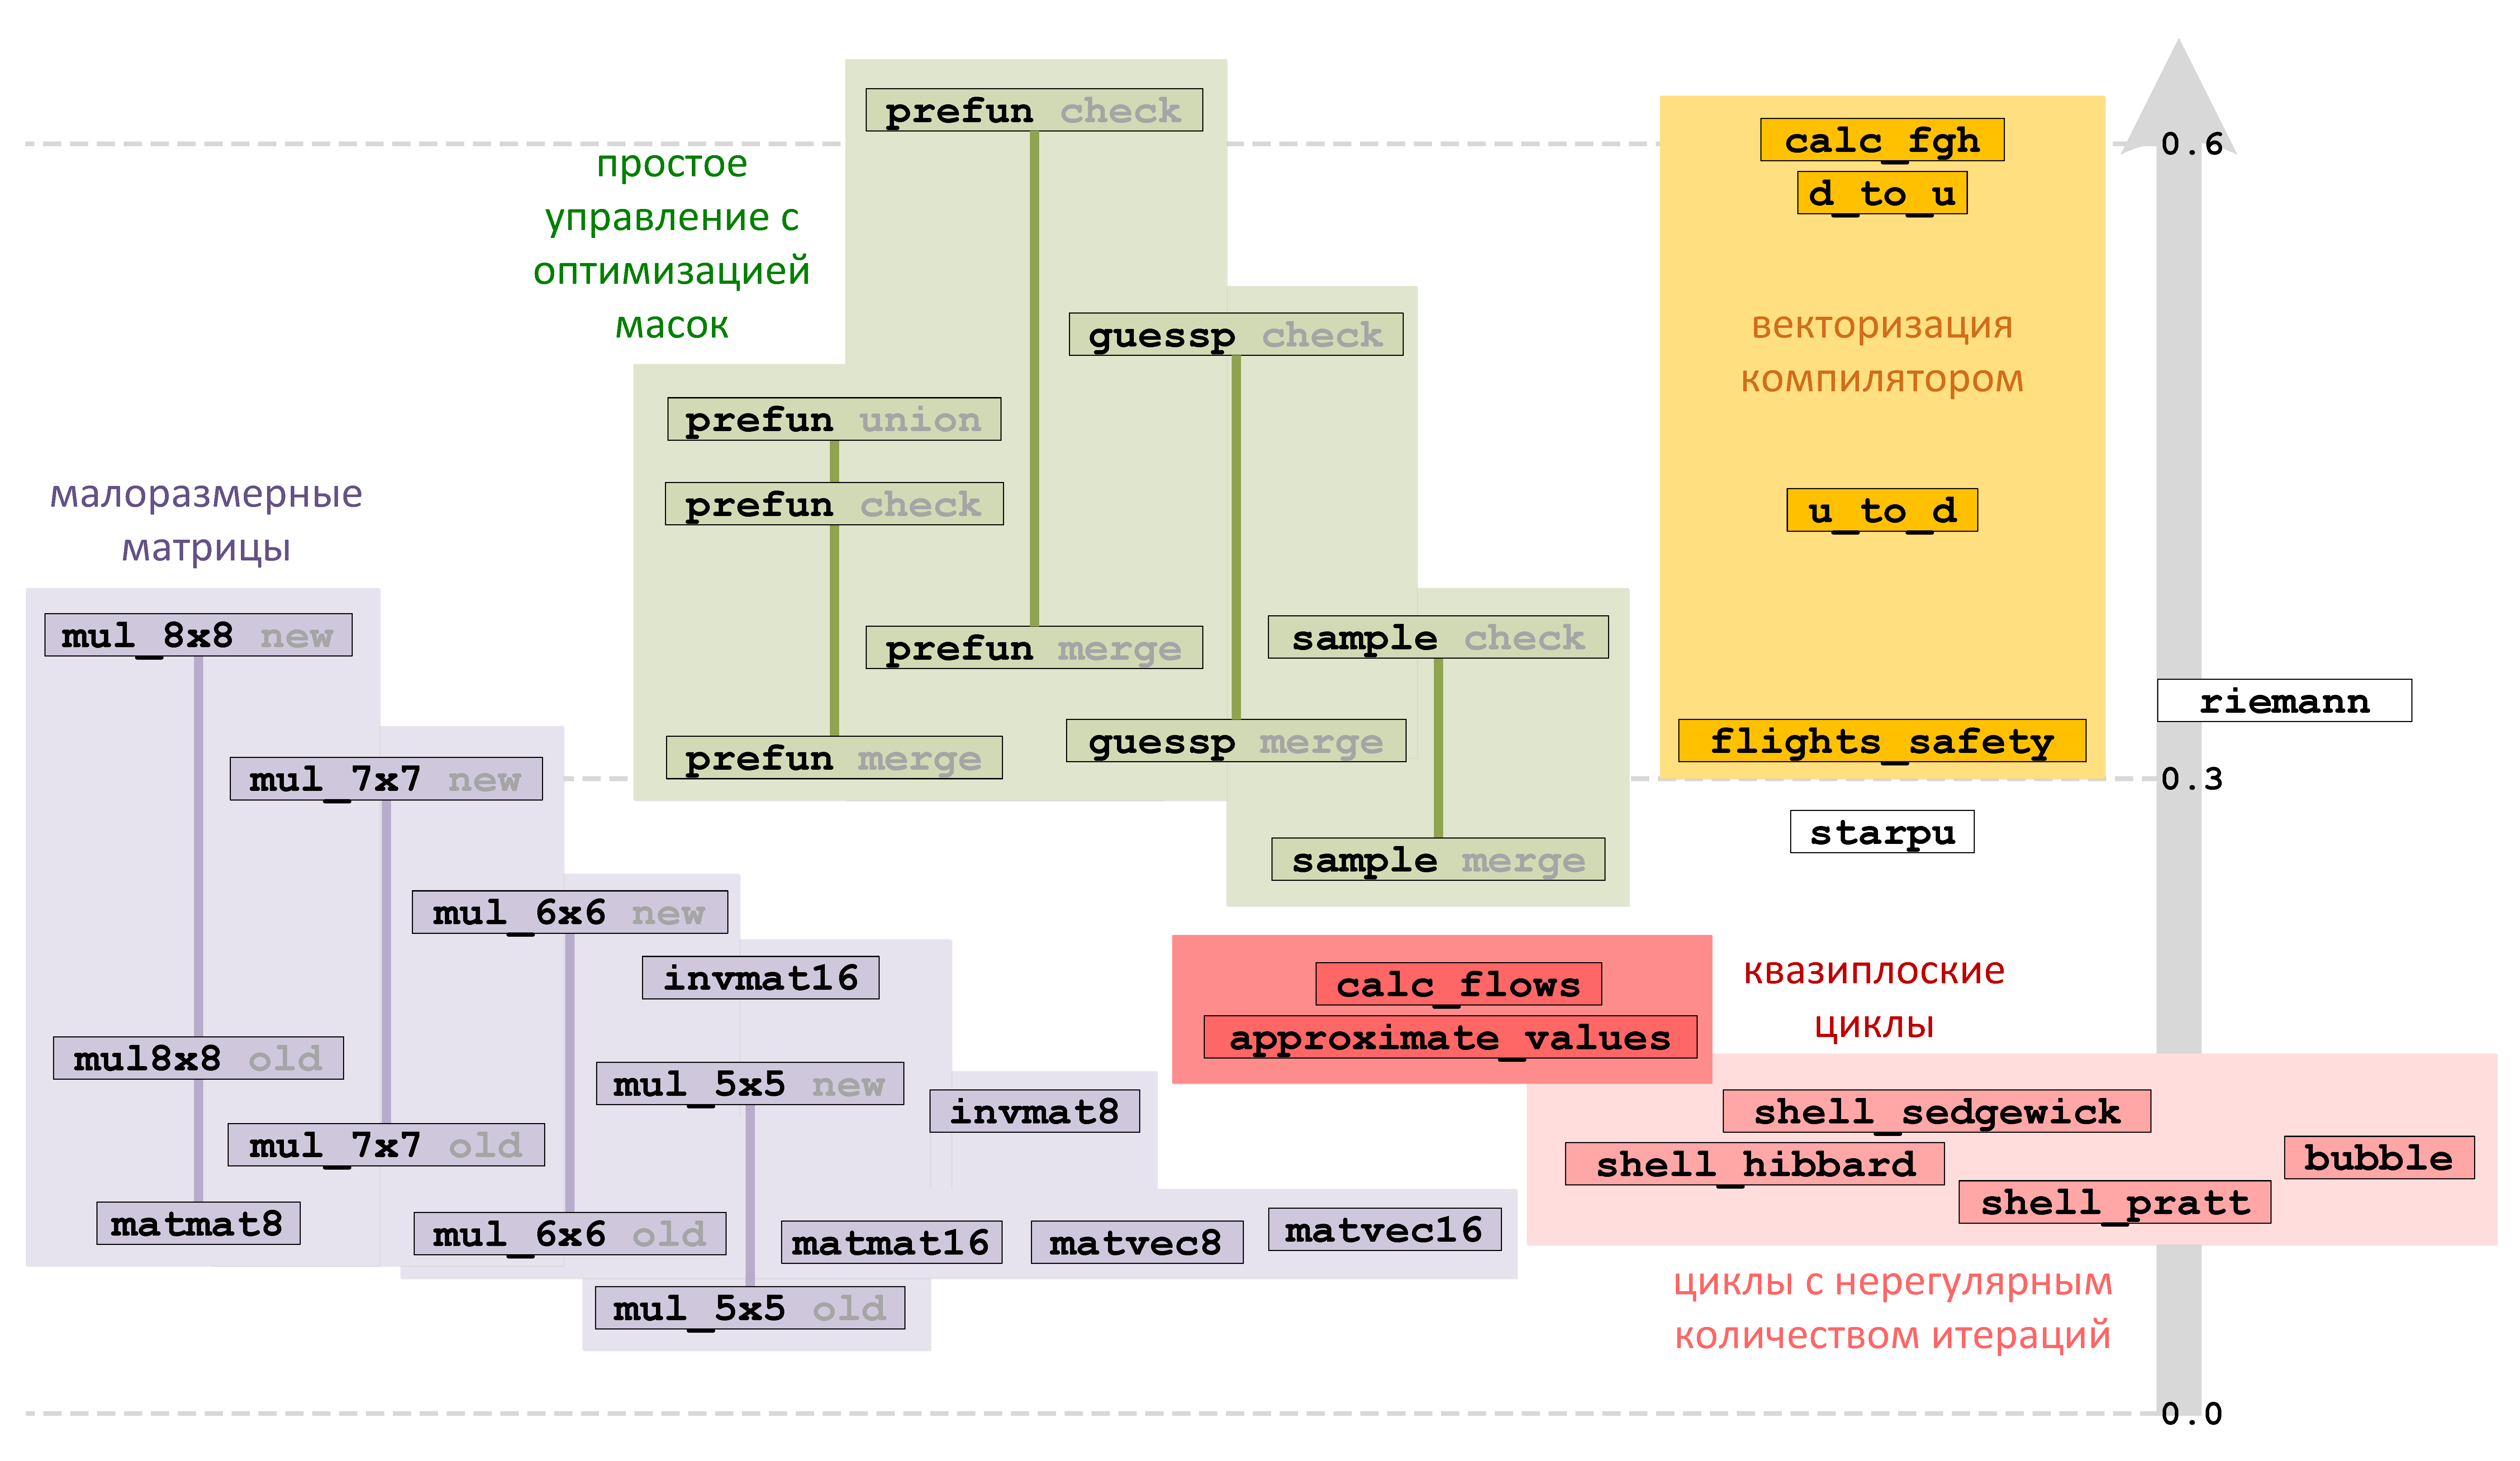
\includegraphics[width=1.0\textwidth]{./pics/text_4_fin/map_cut.pdf}
\singlespacing
\captionstyle{center}\caption{Карта эффективности векторизации.}
\label{fig:text_4_fin_map}
\end{figure}

Векторизация\label{term:vectorization7} является важной низкоуровневой оптимизацией программного кода, с помощью которой можно достичь кратного ускорения суперкомпьютерных приложений.
Все основные современные микропроцессорные архитектуры поддерживают векторные вычисления, причем наблюдается тенденция на увеличение размера вектора (на сегодняшний день максимальная длина равна 512 битам, но уже сейчас логически эта длина не ограничена, учитывая наборы векторных инструкций с переменной длиной вектора).

Сейчас наиболее перспективным набором векторных инструкций является набор AVX-512\label{abbr:avx9}, так как в нем поддержана возможность выборочной обработки элементов векторов с помощью векторных масок\label{term:vector_mask9}.
Эта уникальная возможность позволяет векторизовать сложный программный контекст, содержащий команды передачи управления, гнезда циклов и вызовы функций.

В этой главе были рассмотрены и предложены новые методы векторизации программного кода.
На рис.~\ref{fig:text_4_fin_map} приведена карта сравнения программного контекста различного вида по эффективности векторизации $e_{vec}$.
На этом рисунке схожие по свойствам тестовые примеры объединены в одной цветовой гамме.
Многие из представленных тестовых примеров векторизации программного кода были использованы при численном решении задач обледенения и газовой динамики.

В разделах \ref{sec:text_4_small_matr}, и \ref{sec:text_4_spec_matr} продемонстрированы подходы к векторизации матричных операций малой размерности.
При выполнении векторизации программного кода необходимо уметь находить наборы однотипных операций для объединения их в векторные операции над векторными наборами данных.
При этом полнота использования элементов векторных данных в вычислениях, выраженная в высокой плотности векторных масок\label{term:vector_mask_density7}, напрямую влияет на эффективность векторизации\label{term:vec_eff8} (см. риc.~\ref{fig:text_4_fin_map}, малоразмерные матрицы).

В разделе \ref{sec:text_4_flat} введено понятие плоского цикла\label{term:flat_loop6}, с помощью которого предпринимается попытка унифицировать процесс объединения однотипных операций в векторные инструкции путем записи тела плоского цикла в предикатной форме\label{term:predicate_view5} с последущей векторизацией с помощью замены скалярных операций векторными аналогами.
Можно констатировать, что плоский цикл может быть векторизован при практически произвольном виде его тела (тело может содержать сложное управления, гнезда циклов, вызовы функций).

В разделе \ref{sec:text_4_ibm} приведено описание подхода, как вычисления могут быть представлены в виде композиции плоских циклов с относительно простым телом, после чего успешно векторизованы оптимизирующим компилятором в автоматическом режиме (см. рис.~\ref{fig:text_4_fin_map}, \texttt{calc\_fgh}, \texttt{calc\_d\_to\_u}, \texttt{calc\_u\_to\_d}).
При этом рассматривается предпочтительный способ организации хранения данных в виде <<набора массивов>> и оптимизация расщепления гнезда циклов по условию\label{term:loop_split_by_cond4} для уменьшения количества операций передачи управления внутри плоского цикла.
Отмечено, что цикл, не являющийся в полной мере плоским (квазиплоский цикл)\label{term:flat_kvazy_flat2}, также может быть успешно векторизован, но с некоторой потерей производительности (см. рис.~\ref{fig:text_4_fin_map}, \texttt{calc\_flows}).

Так как основной преградой к эффективной векторизации является наличие операций передачи управления внутри тела плоского цикла (операция передачи управления не может быть векторизована), то в разделе \ref{sec:text_4_loc_branch} рассматриваются оптимизации, направленные на избавление от условий внутри цикла.
Рассматривается оптимизация выноса маловероятного региона из цикла\label{term:meth_vec_del_low_prob_regions3} и поставлен эксперимент по определению эффективности автоматической векторизации при использовании этой оптимизации (см. рис.~\ref{fig:text_4_fin_map}, \texttt{flights\_safety}).
Приведено описание оптимизации <<черная дыра>>\label{term:blackhome_optimization2} по выделению вероятного пути исполнения в теле плоского цикла.

В разделе \ref{sec:text_4_vec_mrg_under_cond} приведено описание и теоретическая оценка общего подхода к избавлению от операций передачи управления и слиянию путей исполнения\label{term:meth_vec_merge4} в теле плоского цикла с помощью векторных инструкций blend.

В разделе \ref{sec:text_4_vec_check_mask} описывается простая операция проверки векторных масок на пустоту\label{term:meth_vec_check4}, которая оказывает наибольший прирост производительности при векторизации простого программного контекста (см. рис.~\ref{fig:text_4_fin_map}, функции с пометкой \texttt{check}).

В разделе \ref{sec:text_4_comb_mask} предлагается метод объединения векторных масок\label{term:meth_vec_union3}, позволяющих одновременно исполнять блоки векторных инструкций с непересекающимися масками (см. рис.~\ref{fig:text_4_fin_map}, \texttt{prefun union}).
Также предлагается метод комбинирования векторных масок\label{term:meth_vec_comb2}, позволяющий одновременно исполнять блоки векторных инструкций с пересекающимися масками.

Остальные разделы посвещены методам векторизации гнезд циклов, в которых один из циклов является плоским.

Наиболее простым случаем является векторизаци гнезда циклов с постоянным количеством итераций, так как в этом случае условие выхода из цикла не требует векторизации.
Этот случай рассмотрен в разделе \ref{sec:text_4_vec_mesh_intersect} и продемонстрировал лучшую эффективность среди примеров векторизации гнезд циклов (см. рис~\ref{fig:text_4_fin_map}, \texttt{tri\_box\_intersect}).

В разделе \ref{sec:text_4_vec_riemann} расмсотрен пример векторизации гнезда циклов с непостоянным количеством итераций для расчетной задачи, в которой условие выхода из цикла на разных итерациях плоского цикла меняется медленно.
Векторизация такого гнезда циклов возможна с помощью векторизации условия выхода из цикла, и эффективность векторизации оказывается ниже, чем в примере с постоянным количеством итераций (см. рис.~\ref{fig:text_4_fin_map}, \texttt{starpu}).

Наиболее сложным для векторизации случаем является векторизация гнезд циклов с нерегулярным количеством итераций.
Такой программый контекст рассмотрен в разделах \ref{sec:text_4_vec_irreg} (вещественные вычисления) и \ref{sec:text_4_integer} (целочисленные вычисления).
При этом внутри итерации плоского цикла векторизуемые условия оказываются непредсказуемыми, что приводит к понижению плотности векторных масок\label{term:vector_mask_density8} в векторных инструкциях и падению производительности (см. рис.~\ref{fig:text_4_fin_map}, циклы с нерегулярным количеством итераций).
Такой программный контекст характерен для дискретных задач и он демонстрирует наиболее низкую эффективность векторизации.

%---------------------------------------------------------------------------------------------------
